\documentclass{article}
\usepackage{hyperref}
\usepackage[margin=1in]{geometry}
\usepackage{indentfirst}
\usepackage{setspace} 
\usepackage{subdepth}
\usepackage{graphicx}
\graphicspath{{./images/}}
\doublespacing


\begin{document}
\title{Regular Languages and Finite-State Machines}
\author{Remington Greko, Tyler Gutowski, Spencer Hirsch, Thomas Johnson}
\date{\today}

\maketitle

\textbf{Regular Expressions and chatGPT}

Give a regular expression that will generate a sequence of natural numbers
that are multiple of 3.

\textit{That is \dots}
\[0, 3, 6, 9, \dots \]

\medskip

\noindent \textit{Solution:} \\
% $\hat{}$(3$\mid$6$\mid$9$\mid$$\backslash$d*(1(01*?0)*?1$\mid$0))\$
$\hat{}$(0*$\mid$(1(01*?0)*?1$\mid$0)\$ \\

According to a question posted on \href{https://stackoverflow.com/questions/4518307/can-i-use-regular-expressions-to-search-for-multiples-of-a-number}{Stack Overflow}
searching for multiples of 48. I was able to conclude that through this search, it would be able to check for multiples of three.
The problem was broken up to see if a number was divisible by both 16 then 3, for our case it is only necessary to check to see if
it is divisible by three. Therefore, I believe that the regular expression listed above is sufficient in solving the problem.

\pagebreak

\textbf{Ask chatGPT to do the same.} \\

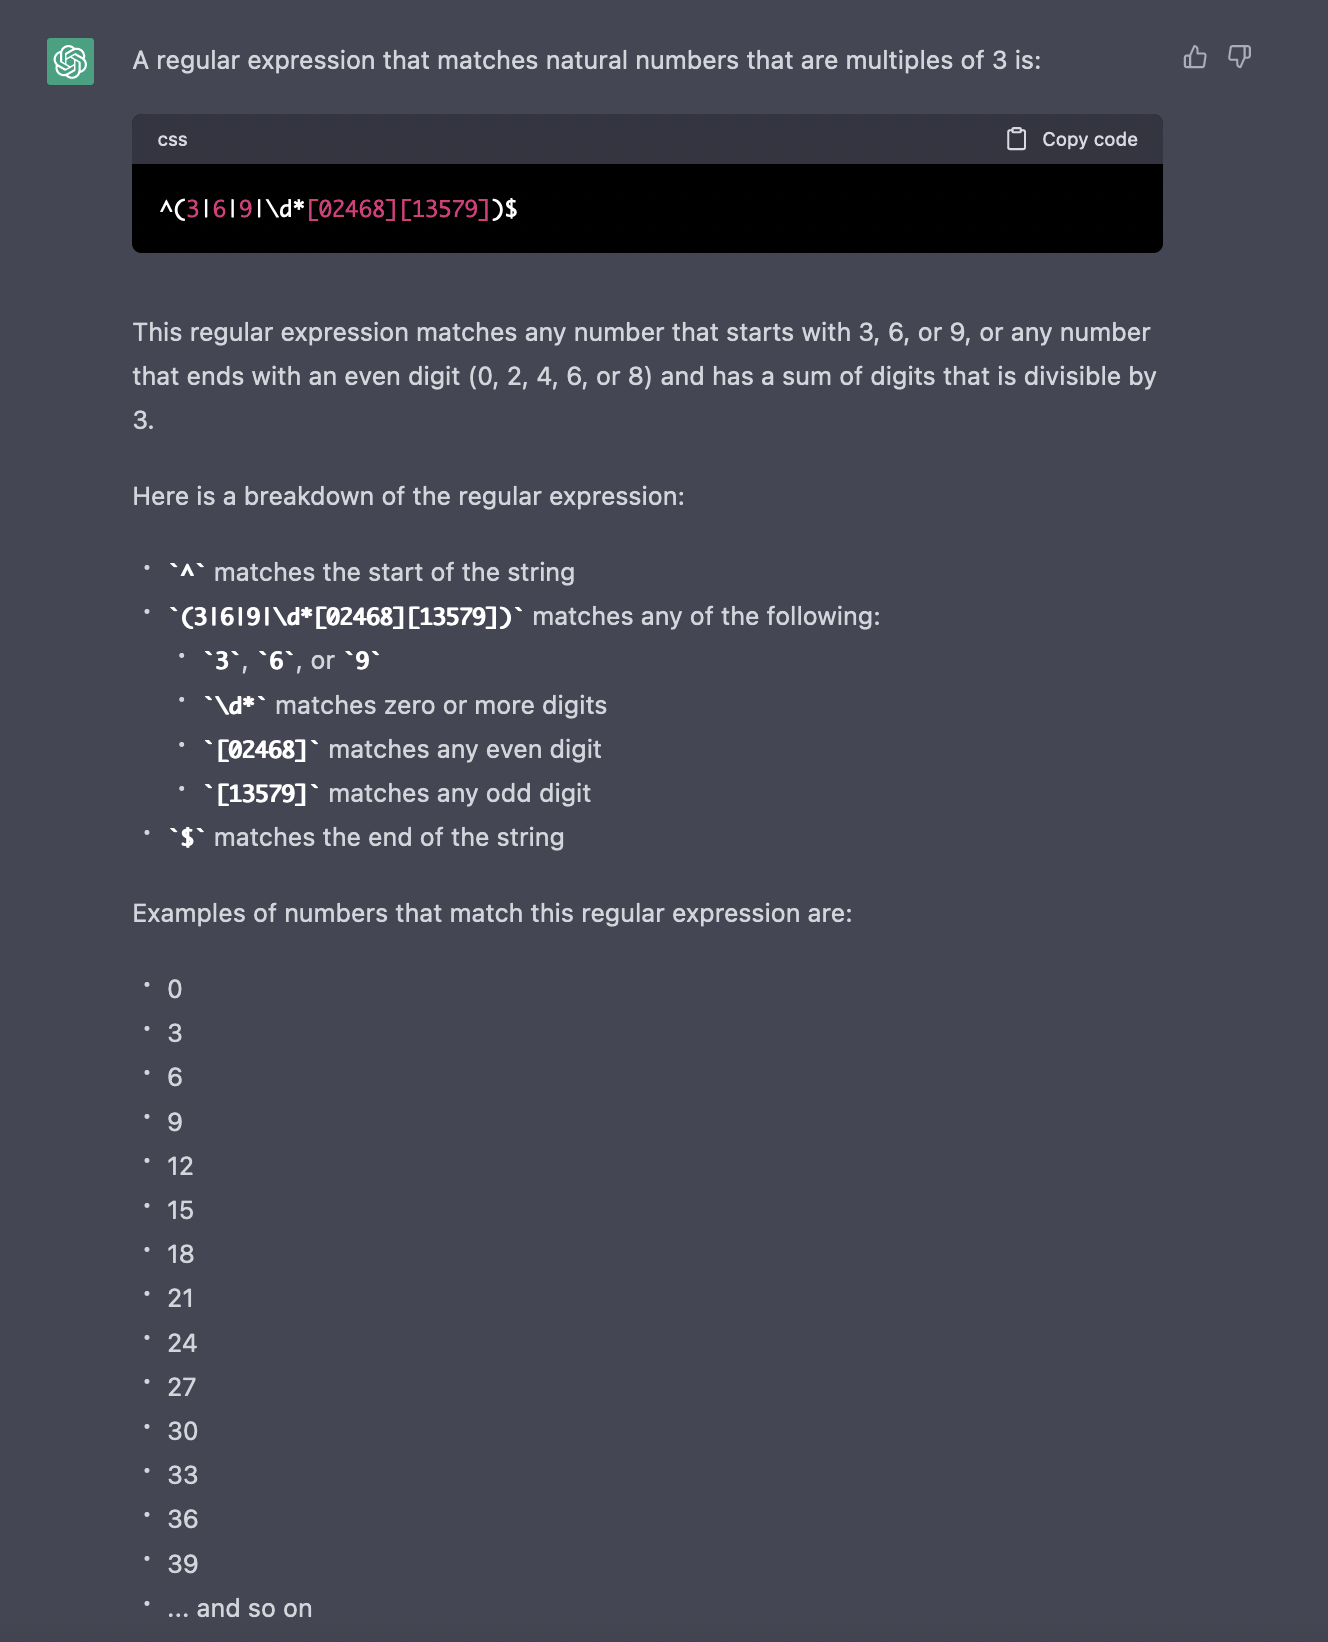
\includegraphics[width=15cm,height=14cm]{chat} \\

\medskip

\end{document}